\begin{chapter}{Theory}
\label{ch:theory}

\section{Generalization of the functional} % (fold)
\label{sec:Generalization of the functional}
The functional defined in (\ref{eq:original_functional}) needs a vector space structure for differences to make sense. Hence, the functional
must be transformed to be still valid in the more general setting of manifold-valued pixels. Since $|x-y|=d(x,y)$ for the 
Euclidean distance on $\mathbb{R}$, the generalization to metric spaces $(X,d)$ is the appropriate way to proceed.\\

To also include the case of 3D pictures and shorten the notation, a graph $G$ is used to specify over which pairs of pixels the sums in (\ref{eq:original_functional})
are taken. Let $V$ be an index set of all pixels in our picture. Denote by $E\subset V\times V$ the set of directed edges in $G$ and by 
$n(i):=\lbrace j\in V: (i,j)\in E\rbrace$ the set of $i$'s neighbors. Then
\begin{align}
    TV_{iso}(u) &= \sum_{i\in V}\sqrt{\sum_{j\in n(i)}d^{2}(u_i,u_j)}\\
    TV_{aniso}(u) &= \sum_{(i,j\in E)}d(u_i,u_j).
\end{align}

Since forward discretization is used, $n(i)$ just contains the next grid neighbors in each dimension, i.e. for $u_i=u((j,k,l))$, the neighbors are 
$n(i)=\lbrace u((j+1,k,l)), u((j,k+1,l)), u((i,k,l+1)) \rbrace$. To also cover inpainting problems, let $V_k\subset V$ be the index set of pixels
where the pixels of the (noisy) original image $u_0$ are known. The generalized functional is given by

\begin{equation}
    \label{eq:general_functional}
    J(u)=\frac{1}{2}\sum_{i\in V_k}d^2(u_i,(u_0)_i) +\lambda TV(u).
\end{equation}


\subsection{The Riemannian distance} % (fold)
\label{sub:RiemannianDistance}
The metric $d$ of course depends on the manifold. Distances on Riemannian manifolds can be measured using smooth curves
$\gamma: [a,b]\to M$ on the manifold. The length of this curve is
\begin{equation}
    L(\gamma) =\int_{a}^b\sqrt{\braket{\dot{\gamma}(t),\dot{\gamma}(t)}_{\gamma(t)}}\mathop{dt},
\end{equation}
where $\braket{\cdot,\cdot}_x$ denotes the inner product on $T_xM$, and the distance can consequently be defined as
\begin{equation}
    d: M\times M\to \mathbb{R},\quad dist(x,y)=\operatorname{inf}_{\Gamma}L(\gamma),
\end{equation}
where $\Gamma$ denotes the set of smooth curves connecting $x,y\in M$. \\

This rather general definition is used by Absil et al \cite{Absil2009} whereas in this thesis Pennec et al's \cite{Arsigny} approach using Riemannian exponential and logarithm map is more convenient. Their definitions are based on
\emph{geodesics} because they are precisely the curves that realize the above minimum.\\

Let $M$ be a connected, geodesically complete Riemannian manifold. The exponential mapping $\exp_x:T_xM\to M$ is defined by $\exp_x(\nu):=\gamma(1)$
where $\gamma:\mathbb{R}\to M$ is the unique geodesic with $\gamma(0)=x$ and $\dot{\gamma}(0)=\nu$.
Thus, the function maps the tangent vector $\nu$ to the point $y$ on the manifold reached after moving along $\gamma$ for $t=1$.
The logarithm map is its inverse and hence yields the tangent vector $\nu$ that belongs to the geodesic connecting $x$ and $y$. \\

A nice overview of Pennec's reinterpretation of vector space operations was given in \cite{mara}.

\begin{table}[h!]
\centering
\begin{tabular}{|l|l|l|}
\hline
Operation   & Vector space &	Riemannian manifold \\
\hline
Subtraction & $\nu=y-x$	& $\nu=\log_x(y)$	\\
Addition    & $y=x+v$	& $y=\exp_x(\nu)$	\\
Distance    & $\operatorname{dist}(x,y)=\norm{y-x}$	& $ \operatorname{dist}(x,y)=\norm{\log_x(y)}_x$ \\
\hline
\end{tabular}
\caption[Comparison vector space and manifold operations]{reinterpretation of vector space operations on Riemannian mannifolds}
\end{table}
% subsection The Riemmanian distance (end)
% section Generalization of the functional (end)

\section{Algorithms} % (fold)
\label{sec:Algorithms}
The next topic that must be addressed is the minimization of the above defined functional. It brings about another challenge in the form of its non-differentiability.
In the implementation, this problem is solved using two different methods. They are based on either working with a regularized version of the functional or by so-called
proximal mappings. The latter is used by the proximal point algorithm which will be shortly summarized in the next section before proceeding to
the iteratively reweighted least squares (IRLS) algorithm.


\subsection{Proximal point} % (fold)
\label{sub:ProximalPoint}
The proximal point algorithm for manifold-valued data which is implemented in the MTVMT library is based on the work of Weinmann et al\cite{Weinmann} and belongs to the class
of proximal splitting methods. A survey on these methods for Euclidean space data is provided in \cite{CombettesPequet}. The general scope in the real case are convex
optimization problems of the form
\begin{equation}
    \text{minimize}_{x\in \mathbb{R}^n} f_1(x) + \cdots +f_m(x)
\end{equation}
where the $f_i:\mathbb{R}^n\to]-\infty,\infty]$ are convex functions but not necessarily differentiable. This is also true for the functional (\ref{eq:general_functional}),
even for the simple Euclidean case where the summands are given by $d(x,y)=|x-y|$. \\
Splitting means considering every summand $f_i$ individually and minimizing it using its proximal mapping
\begin{equation}
    \label{eq:real_proximity}
    \operatorname{prox}_{f_i}x=\operatorname{argmin}_{y\in\mathbb{R}^n}\left(f_i(y) + \frac{1}{2}\norm{x-y}^2_{2} \right).
\end{equation}
For the case of a differentiable function $f$, the minimization problem (\ref{eq:real_proximity}) 
can be written in an explicit form such that $\operatorname{prox}_f x = x-\nabla f$, which 
can be interpreted as a gradient descent step.\\
In addition to that, one can show that the minimizers of $f$ are exactly the fixed points of the proximal mapping (See \cite{ParikhBoyd}, \S 2.3).

\subsubsection{Application to manifolds} % (fold)
\label{ssub:Application to manifolds}
Let $M$ be a Riemannian manifold and $\Omega$ as defined in \ref{sub:Discretization}. Due to the square root involved in the isotropic case,
the method can only be applied to the anisotropic version of the functional (\ref{eq:general_functional}) and leads in the 2D case to the following splitting
\begin{align}
    J(u)	&= \sum_{i,j}F_{ij}(u)+\lambda\sum_{i,j}G_{ij}(u)+\lambda\sum_{i,j}H_{ij}(u)\\
    F_{ij}(u)	&=  d^{2}(u_{i,j},(u_0)_{i,j})\\
    G_{ij}(u)	&=  d(u_{i,j},u_{i,j+1})\\
    H_{ij}(u)	&=  d(u_{i,j},u_{i+1,j})
\end{align}
and proximal mappings of the form
\begin{equation}
\label{eq:manifold_proximity}
\operatorname{prox}_{\lambda G_{ij}}x=\operatorname{argmin}_{y\in M^{m\times n}}\left(\lambda G_{ij}(y) +\frac{1}{2}d^2(x,y) \right).
\end{equation}

Only the expressions relevant for the implementation and the algorithm itself are presented in the following. For details on derivations and convergence and existence proofs consider \cite{Weinmann}.\\

The proximal mappings itself can be computed using unit speed geodesics. Here $[x,y]_t$ denotes the point reached by
following the unit speed geodesic starting at $x$ in direction $y$ for a time $t$.
\begin{align}
    (\operatorname{prox}_{\lambda G_{ij}}u)_{ij}&=[u_{i,j},u_{i,j+1}]_{t_{TV}} \\
    (\operatorname{prox}_{\lambda H_{ij}}u)_{ij}&=[u_{i,j},u_{i+1,j}]_{t_{TV}} \\
    (\operatorname{prox}_{\lambda F_{ij}}u)_{ij}&=[u_{i,j},(u_0)_{i,j}]_{t_{l^2}}
\end{align}

Lastly, the times in the case of $G_{ij}$ and $F_{ij}$ are computed by
\begin{align}
    t_{TV}&=
    \begin{cases}
	\mu, &\text{if } \mu<d(u_{i,j},u_{i,j+1})\\
	\mu<d(u_{i,j},u_{i,j+1}), & \text{else}
    \end{cases}\\
    t_{l^{2}}&=\frac{\mu}{1+\mu}d(u_{i,j},(u_0)_{i,j})
\end{align}
and for $H_{ij}$ analogously.\\

In summary, the parallel version of the proximal algorithm now works by computing a proximal mapping for every pixel $u_{i,j}$.
The relevant geodesics are in direction of its next neighbors on the grid and in direction of the corresponding pixel of the original picture $u_0$, i.e. $[u_{i,j}, v]_t$ with $v\in\lbrace u_{i-1,j},u_{i+1,j},u_{i,j-1}, u_{i,j+1}, (u_0)_{i,j}\rbrace$. Next, the intrinsic (Karcher) mean \cite{Karcher} of 
these five mappings is computed and the pixel is updated to a new value $u_{i,j}'$.\\

Finally, the algorithm is stated in Algorithm \ref{al:parallel_prpt}.

\begin{algorithm}
\caption{Parallel proximal point algorithm}
\label{al:parallel_prpt}
\begin{algorithmic}
\REQUIRE $\mu =(\mu_1,\mu_2, \ldots)\in l^2\setminus l^1$
\STATE $u \leftarrow u_0$
\FOR{$r\leftarrow 1,2,\ldots$} 
\FOR{$i\leftarrow 1,2,\ldots,m;$ $j\leftarrow 1,2,\ldots,n;$} 
\STATE $t \leftarrow t_{l^{2}}=\frac{\mu_r}{1+\mu_r}d(u_{i,j},(u_0)_{i,j})$
\STATE $z^{(1)} \leftarrow [u_{i,j},(u_0)_{i,j}]_t$
\STATE $t \leftarrow  t_{TV}(\mu_r\lambda,u_{i,j},u_{i,j+1})$
\STATE $z^{(2)} \leftarrow [u_{i,j},u_{i,j+1}]_t$
\STATE $t \leftarrow  t_{TV}(\mu_r\lambda,u_{i,j},u_{i,j-1})$
\STATE $z^{(3)} \leftarrow [u_{i,j},u_{i,j-1}]_t$
\STATE $t \leftarrow  t_{TV}(\mu_r\lambda,u_{i,j},u_{i,j+1})$
\STATE $z^{(4)} \leftarrow [u_{i,j},u_{i,j+1}]_t$
\STATE $t \leftarrow  t_{TV}(\mu_r\lambda,u_{i,j},u_{i-1,j})$
\STATE $z^{(5)} \leftarrow [u_{i,j},u_{i-1,j}]_t$
\STATE $u'_{i,j} \leftarrow$ karchermean($z^{(1)},z^{(2)},z^{(3)},z^{(4)},z^{(5)}$)
\ENDFOR
\FOR{$i\leftarrow 1,2,\ldots,m;$ $j\leftarrow 1,2,\ldots,n;$}
\STATE $u_{i,j} \leftarrow u'_{i,j}$
\ENDFOR
\ENDFOR
\end{algorithmic}
\end{algorithm}

% subsubsection  (end)
% subsubsection Application to manifolds (end)

% subsection Proximal Point (end)

\subsection{Iteratively reweighted least squares} % (fold)
\label{sub:IRLS}
The IRLS approach to dealing with non-differentiable terms in the functional is by adding additional terms for regularization. In the continuous (and isotropic) case that means
\begin{equation}
    \label{eq:regulzarized_tv}
    TV_{\epsilon}=\int_{\Omega}\omega_{\epsilon}|\nabla u|^2 =\int_{\Omega}\frac{|\nabla u|^2}{\sqrt{|\nabla u|^2+\epsilon^2}}
\end{equation}
for a small $\epsilon>0$. In this form, the functional becomes differentiable but directly minimizing a
regularized functional $J_{\epsilon}$ will not work either.\\

The IRLS algorithm, described in more detail in \cite{Rodriguez}, works by alternating between reweighting and minimization steps. First, the weights are computed then 
the minimization is performed using the regularized functional with the weights considered constant.
 The steps for the isotropic functional are as follows
\begin{align}
    w_{i}^{new} &= W^{\epsilon}_{iso}(u)_i := \left( \sum_{j\in n(i)}d(u_i,u_j)+\epsilon^2\right)^{-\frac{1}{2}}\; \forall\;i\in V \\
    u^{new} &= U(w) := \operatorname{argmin}_{u\in\Omega}\sum_{i\in V_k}d^2(u_i,(u_0)_{i})+\lambda\sum_{i\in V}w_i\sum_{j\in n(i)}d^2(u_i,u_j).
\end{align}
The anisotropic steps are
\begin{align}
    w_{i,j}^{new} &= W^{\epsilon}_{aniso}(u)_{i,j} := \left( d(u_i,u_j)+\epsilon^2\right)^{-\frac{1}{2}},\; \forall\;(i,j)\in E \\
    u^{new} &= U(w) := \operatorname{argmin}_{u\in\Omega}\sum_{i\in V_k}d^2(u_i,(u_0)_{i})+\lambda\sum_{(i,j)\in E}w_{i,j}d^2(u_i,u_j).
\end{align}

Further details on the derivation and proofs on convergence, existence and uniqueness of solutions for different manifold classes, such as Hadamard spaces or the sphere,
can be found in \cite{SprecherIRLS}. The minimization can in principle be performed using various methods from smooth optimization theory. Due to its quadratic
convergence rate, here the Newton method was chosen. The algorithm is stated in Algorithm \ref{al:parallel_irls}. 

\begin{algorithm}
\caption{IRLS algorithm}
\label{al:parallel_irls}
\begin{algorithmic}
\STATE Choose initial value $u^{(0)}$ by application of smoothing filter on $u_0$
\STATE $i\leftarrow 0$
\REPEAT
\STATE $W \leftarrow W^{\epsilon}(u^{(i)})$
\STATE $u^{(i,0)} \leftarrow u^{(i)}$
\STATE $k\leftarrow 0$
\REPEAT
\STATE $u^{(i,k+1)}=newtonstep^{\lambda,u_0,V_k,V,E}(W,u^{(i,k)})$
\STATE $k\leftarrow k+1$
\UNTIL{Stopping criteria (e.g. $k=1, J(u^{(i,k+1)})<J(u^{(i,0)}),d(u^{(i,k+1)},u^{(i,k)}}$)
\STATE $u^{(i+1)} \leftarrow u^{(i,k+1)}$
\STATE $i\leftarrow i+1$
\UNTIL{$d(u^{(i+1)},u^{(i)})<tol$}
\RETURN $u^{(i+1)}$
\end{algorithmic}
\end{algorithm}
% subsection IRLS (end)
% section Algorithms (end)

\section{Riemannian Newton method} % (fold)
\label{sec:Riemannian Newton method}
In numerical analysis, the Newton method is one of the standard algorithms for finding approximations of roots of real-valued functions. Due to its locally at least quadratic
convergence, the algorithm or one of its numerous variants and generalizations is used in many applications. For its application in optimization, the Newton method is applied to the gradient of the objective function which also requires the evaluation of its Hessian.
The following section provides a short summary of the generalization of gradient and Hessian to a manifold setting.

\subsection{Gradient} % (fold)
\label{sub:Gradient}
Let $M$ be a Riemannian manifold and $T_xM$ the tangent space at $x\in M$. Furthermore, let $f: M\to\mathbb{R}$ be a smooth function defined on $M$.
Define the \emph{Riemannian gradient} $\operatorname{grad} f$ to be the unique tangent vector $\xi\in T_xM$ satisfying 
\begin{equation}
    \label{eq:gradient}
    \braket{\operatorname{grad}f(x),\xi}_x=\mathop{Df}(x)[\xi]
\end{equation}
where $\mathop{Df}(x)[\xi] = \xi[f]$, when $\xi:\mathcal{C}^{\infty}(M)\to\mathbb{R}$ is interpreted as derivation acting on $f$. The Riemannian gradient
shares many properties of its Euclidean counterpart, in particular defining the direction of steepest ascent, such that first order methods like
gradient descent could already be implemented at this point.\\
% subsection Gradient (end)

\subsection{Hessian} % (fold)
\label{sub:Hessian}
For second order methods, such as the Newton algorithm, also a corresponding \emph{Riemannian Hessian} is needed. Following again the work 
of Absil et al \cite{Absil2009}, the Hessian is realized as linear endomorphism of the tangent space $T_xM$
\begin{equation}
    \label{eq:hessian}
    \operatorname{Hess}f(x)[\xi]=\nabla_{\xi}\operatorname{grad}f(x),
\end{equation}
where $\nabla$ denotes the Riemannian connection on $M$.\\
% subsection Hessian (end)

\subsection{Newton equation} % (fold)
\label{sub:Newton equation}
Now let $x\in M$ and $\gamma:[a,b] \to M$ be the unique geodesic with $\gamma(0)=x$ and $\dot{\gamma}(0)=\nu\in T_xM$ 
passing through $y\in M$. Thus, one can set $y=\exp_x(\nu)$ and $\nu=\log_x(y)$ as suggested in \ref{sub:RiemannianDistance}. Using the
definitions of gradient and Hessian above one can expand $f$ to second order around $x$ in the following way
\begin{align}
    \label{eq:manifold_taylor}
    f(\exp_x(\nu)) &= f_x(\nu) = f(x) + \braket{\operatorname{grad}f(x),\nu}_x + \frac{1}{2}\braket{\operatorname{Hess}f(x)[\nu],\nu}_x + \mathcal{O}(\norm{\nu}_x^3)\quad \Leftrightarrow \\
    f(y) &= f(x) + \braket{\operatorname{grad}f(x),\log_x(y)}_x + \frac{1}{2}\braket{\operatorname{Hess}f(x)[\log_x(y)],\log_x(y)}_x + \mathcal{O}(\norm{\log_x(y)}_x^3).\nonumber
\end{align}

The first line of (\ref{eq:manifold_taylor}) suggests that, for given fixed $x$, $f$ can also be interpreted as a function of $\nu\in T_xM$ and the optimization of $f$ can be 
performed on the tangent space, on which $\operatorname{grad}f$ and $\operatorname{Hess}f$ have been defined. 
This finally leads to the following generalization of the \emph{Newton equation}
for the correction term $\eta_x \in T_xM$:
\begin{equation}
    \label{eq:newtoneq}
    \operatorname{Hess}f(x)[\eta_x]=-\operatorname{grad}f(x)
\end{equation}

The solution of the Newton equation $\eta_x$ is a tangent vector of $T_xM$ and, as (\ref{eq:manifold_taylor}) already implies, can be mapped back to the manifold $M$ 
using the exponential map such that $y'=\exp_x(\eta_x)$. The whole iterative procedure, based on \cite{Absil2009}, Algorithm 5, is summarized in the following listing.
\begin{algorithm}
\caption{Riemannian Newton method for real-valued functions}
\label{al:real_riemannian_newton}
\begin{algorithmic}
\STATE $x_0 \leftarrow x\in M$ (initial value)
\FOR{$k\leftarrow 0,1,2 \ldots$} 
\STATE Solve newton equation $\operatorname{Hess} f(x_k)\eta_k = -\operatorname{grad} f(x_k)$ for $\eta_k\in T_{x_k}M$
\STATE $x_{k+1} \leftarrow \exp_{x_k}(\eta_k)$
\ENDFOR
\end{algorithmic}
\end{algorithm}
% subsection Newton equation (end)

\subsection{Newton equation for the TV functional} % (fold)
\label{sub:NewtonequationfortheTVfunctional}
Next, the general form of the linear system defined by (\ref{eq:newtoneq}) in the case of manifold-valued 3D images $u,u_0: \Omega\to M^{Z\times Y\times X}$
where $\Omega=\lbrace 1,\ldots, Z\rbrace\times\lbrace 1,\ldots, Y\rbrace\times\lbrace 1,\ldots, X\rbrace$ for $X,Y,Z\in\mathbb{N}$ and a corresponding functional $J:  M^{Z\times Y\times X} \to \mathbb{R}$ is shown.
Furthermore, the forward finite difference scheme described in \ref{sub:Discretization} is used. To simplify notation,
assume the regularization weights obtained from the last IRLS reweighting step to be all equal to $1$ and thus consider only the
bare $d^2(\cdot,\cdot)$ terms:
\begin{align}
    & J(u_{111},u_{112},\ldots,u_{ijk},\dots,u_{ZYX}) = \sum_{ijk} d^2(u_{ijk},(u_0)_{ijk}) \\ 
    &+ \lambda \sum_{ijk}^{Z-1,Y,X}d^{2}(u_{ijk},u_{i+1,j,k}) 
    + \lambda \sum_{ijk}^{Z,Y-1,X}d^{2}(u_{ijk},u_{i,j+1,k}) 
    + \lambda \sum_{ijk}^{Z,Y,X-1}d^{2}(u_{ijk},u_{i,j+1,k}). \nonumber 
\end{align}

The first derivatives are given by the following expressions
\begin{align}
    \label{eq:funcfirstder}
    \frac{\partial J}{\partial u_{mnp}} = d^2_x(u_{mnp},(u_0)_{mnp}) &+ \lambda 
	\big(
	    d_x^2(u_{mnp},u_{m+1,n,p}) +  d_y^2(u_{m-1,n,p},u_{mnp}) \\
	  &+  d_x^2(u_{mnp},u_{m,n+1,p}) +  d_y^2(u_{m,n-1,p},u_{mnp}) \nonumber \\
	  &+  d_x^2(u_{mnp},u_{m,n,p+1}) +  d_y^2(u_{m,n,p-1},u_{mnp})\big), \nonumber 
\end{align}
where $d^2_x((u,v)):=\frac{\partial}{\partial x}\left. d^2(x,y)\right\vert_{(x,y)=(u,v)}$.\\

The second derivatives, considering only the terms in the first line of (\ref{eq:funcfirstder}) containing the fidelity term and discrete gradient components in $z$ direction, are then
\begin{align}
    \label{eq:funcsecder}
    \frac{\partial^2 J}{\partial u_{ijk}\partial u_{mnp}} &=  \delta_{nj}\delta_{kp}\delta_{mi}d^2_{xx}(u_{ijk},(u_0)_{ijk}) \\
    &+\lambda\delta_{nj}\delta_{kp}
    \bigg[ 
	\delta_{mi} \bigg(d_{xx}^2(u_{ijk},u_{i+1,j,k}) +d_{yy}^2(u_{ijk},u_{i+1,j,k}) \bigg)\\
    &+  \delta_{m-1,i}d_{xy}^2(u_{ijk},u_{i+1,j,k}) +\delta_{m+1,i} d_{yy}^2(u_{i-1,j,k},u_{ijk})
    \bigg].
\end{align}
Considering the pattern of the Kronecker deltas and reshaping the tensor of second partial derivatives into a single matrix, one 
obtains a block-band matrix, where sums of non-mixed second derivatives of the squared distance function are located on the main diagonal, while all mixed
derivatives belonging to the same gradient component ($x,y$ or $z$) populate subdiagonals of equal distance to the main diagonal.
In particular, discretizations in $x$-direction are on the first, in $y$-direction on the $X$th and in $z$-direction on the $X\times Y$th subdiagonals.\\

To illustrate this, consider the following schematic of the band structure

\begin{equation}
    HJ=
\begin{pmatrix}
D	& X	    & 		& Y	    & 		& Z	    & 	   \\
X	& D	    & X		& 	    & Y		& 	    & Z	  \\
	& X	    & D	    & X	    & 		& Y	    & 	 \\
Y	& 	    & X		& D	    & X		& 	    & Y	\\
	& Y	    & 		& X	    & D		& X	    & 	\\
Z	& 	    & Y		& 	    & X		& D	    & X	\\
	& Z	    & 		& Y	    & 		& X	    & D	\\
\end{pmatrix},
\end{equation}
where $D$ denotes a block, consisting of the sum of non-mixed second derivatives, according to the rules defined by the generalization of (\ref{eq:funcsecder}) to all 
discretization directions.\\

$HJ$ is exactly the matrix representation of the Hessian operator $\operatorname{Hess}J(u)$, while the representation $GJ$ of $\operatorname{grad}J(u)$ is just the vectorized version
of the tensor of first derivatives (\ref{eq:funcfirstder}). If the embedding space of the manifold is given by $\mathbb{R}^{n\times p}$ then the matrix $HJ$
will be an element of $\mathbb{R}^{\tilde D\times\tilde D}$ with $\tilde D=npXYZ$. $HJ$ is, however, also sparse with approximately $7\tilde D$ non-zero entries.
Finally, solving the Newton equation (\ref{eq:newtoneq}) corresponds to solving the sparse linear system given by $HJ$ and $GJ$, which is also the most computationally demanding
part of the algorithm.

% subsection Newton equation for the TV functional (end)
\subsection{Tangent space restriction} % (fold)
\label{sub:Tangent space restriction}
Lastly, a basis of the tangent space $T_xM$ for each $x\in M$ can be chosen such that the computed gradient and Hessian are restricted to the tangent space by performing a basis transformation. Since $\operatorname{dim}T_xM=\operatorname{dim} M$, this means that tangent vectors, such as the gradients 
of the squared distance function, or tangent space mappings, like the Hessian, can be expressed using only $\operatorname{dim} M$ coefficients. Now $D=\operatorname{dim}M (XYZ)$ such that the prefactor is the intrinsic manifold dimension and not the dimension of the embedding space any more.

% subsection Tangent space restriction (end)

% section Riemannian Newton method (end)

\section{Manifolds} % (fold)
\label{sec:Manifolds}
In this section all relevant quantities to implement the IRLS and proximal point algorithm are presented. These are the distance function and its derivatives,
exponential and logarithm mapping and the tangent space basis transformation mapping. 
For the Grassmann manifold, due to its quotient manifold nature and because it was not covered in the original implementation based on \cite{SprecherIRLS}
a more general introduction will be given.

\subsection{Euclidean space} % (fold)
\label{sub:Euclidian}
The space in question is just $\mathbb{R}^n$, hence trivially a manifold and naturally a vector space such that all expressions can be calculated using basic
multivariable calculus. The exponential and logarithm mappings are not to be understood in the sense of $e^x$ but according to \ref{sub:RiemannianDistance} such that
they are just addition and subtraction in the vector space.

\subsubsection{Exponential map} % (fold)
\label{ssub:ExponentialEUC}
\begin{equation}
    \exp_x(r)=x+r    
\end{equation}
% subsubsection Exponential map (end)

\subsubsection{Logarithm map} % (fold)
\label{ssub:LogarithEUC}
\begin{equation}
    \log_x(y)=y-x
\end{equation}
% subsubsection Logarithm map (end)

\subsubsection{Squared distance function} % (fold)
\label{ssub:SquareddistanceEUC}
\begin{equation}
    d(x,y)=\norm{x-y}^{2}=\sum_{i=1}^n(x_i-y_i)^{2}
\end{equation}
% subsubsection Squared distance function (end)

\subsubsection{First derivative of the squared distance function} % (fold)
\label{ssub:FirstDerEUC}
\begin{equation}
    \frac{\partial d^2(x,y)}{\partial y}=2x
\end{equation}
% subsubsection First derivative of the squared distance function (end)

\subsubsection{Second derivatives of the squared distance function} % (fold)
\label{ssub:SecondDerEUC}
\begin{equation}
    \frac{\partial^2 d^2(x,y)}{\partial x\partial y}=\frac{\partial^2 d^2(x,y)}{\partial x^2}=2\mathbbm{1}_n;
\end{equation}
where here and in all following expression $\mathbbm{1}_n$ denotes the identity matrix.


% subsubsection Second derivatives of the squared distance function (end)
\subsubsection{Tangent space restriction map} % (fold)
\label{ssub:TangentEUC}
\begin{equation}
    T_x=\mathbbm{1}_{n^2}
\end{equation}
% subsubsection Tangent space restriction map (end)

% subsection Euclidian (end)

\subsection{Sphere $S^n$} % (fold)
\label{sub:Sphere}
Consider the manifold $S^n:=\lbrace x\in\mathbb{R}^{n+1}: \norm{x}=1\rbrace\subset\mathbb{R}^{n+1}$ and express the maps in terms of vectors $x,y\in\mathbb{R}^{n+1}$ of the Euclidean 
embedding space.\\
The tangent space $T_xS^n$ at $x\in\mathbb{R}$ is, as basic intuition suggests, given by the tangent hyperplane to the sphere at $x$ such that
\begin{equation}
    \label{eq:sntangentspace}
    T_xS^n:=\lbrace y\in\mathbb{R}^{n+1}: x^Ty=0 \rbrace
\end{equation}
The standard Euclidean inner product $\braket{r,s}=r^Ts$, restricted to the tangent space, turns $S^n$ into a Riemannian manifold.

\subsubsection{Exponential map} % (fold)
\label{ssub:ExponentialS2}
\begin{equation}
    exp_x(r)= \cos(\norm{r}_2)x + \frac{\sin(\norm{r}_{2})}{\norm{r}_{2}}r 
\end{equation}
% subsubsection Exponential map (end)

\subsubsection{Logarithm map} % (fold)
\label{ssub:LogarithmS2}
\begin{equation}
    \log_x(y)= \arccos(x^Ty)\frac{y-x^Tyx}{\norm{y-x^Tyx}_2}
\end{equation}
Note that this is only well-defined for non-antipodal points $x,y\in S^n$.
% subsubsection Logarithm map (end)

\subsubsection{Squared distance function} % (fold)
\label{ssub:SquareddistanceS2}
\begin{equation}
    d(x,y)=\arccos(x^Ty)
\end{equation}
% subsubsection Squared distance function (end)

\subsubsection{First derivative of the squared distance function} % (fold)
\label{ssub:FirstDerS2}
\begin{equation}
    \frac{\partial d^2(x,y)}{\partial x}=\begin{cases}
	\frac{-2\arccos(x^Ty)}{\sqrt{1-(x^Ty)^{2}}}y, & x^Ty\in (-1,1)\\
	-2y, & x^Ty=1
    \end{cases}
\end{equation}
% subsubsection First derivative of the squared distance function (end)

\subsubsection{Second derivatives of the squared distance function} % (fold)
\label{ssub:SecondDerS2}
\begin{equation}
    \frac{\partial^2 d^2(x,y)}{\partial x^2}=\begin{cases}
	\bigg[\frac{2}{1-(x^Ty)^2}-\frac{2\arccos(x^T)}{(1-(x^Ty)^{2})^{\frac{3}{2}})}x^Ty\bigg]yy^T+2x^Ty\;\mathbbm{1}_{n+1}, & x^Ty\in(-1,1)\\
	\frac{2}{3}yy^T+2x^Ty\mathbbm{1}_{n+1}, & x^Ty=1
    \end{cases}
\end{equation}
And the mixed derivative:
\begin{equation}
    \frac{\partial^2 d^2(x,y)}{\partial x\partial y}=\begin{cases}
	\bigg[\frac{2}{1-(x^Ty)^2}-\frac{2\arccos(x^Ty)}{(1-(x^Ty)^{2})^{\frac{3}{2}}}x^Ty\bigg]yx^T-\frac{-2\arccos(x^Ty)}{\sqrt{1-(x^Ty)^{2}}}y\;\mathbbm{1}_{n+1} , & x^Ty\in(-1,1)\\
	\frac{2}{3}yx^T -2\;\mathbbm{1}_{n+1}, & x^Ty=1
    \end{cases}
\end{equation}

% subsubsection Second derivatives of the squared distance function (end)

\subsubsection{Tangent space restriction map} % (fold)
\label{ssub:TangentS2}
As implied by (\ref{eq:sntangentspace}), the tangent space $T_xS^n$ at $x\in S^n$ is just the orthogonal complement of $x$ in $\mathbb{R}^{n+1}$.
Thus, constructing a basis of the tangent space amounts to constructing an orthonormal basis $\lbrace b_0,b_1,\cdots,b_n\rbrace$ of $\mathbb{R}^{n+1}$ with $b_0=x$. Then
$\mathcal{B}=\lbrace b_i\rbrace_{i=1}^{n}$ is the basis of the tangent space.\\
This can be done using the QR algorithm or, in the case of $S^2\subset\mathbb{R}^3$, using the cross product. For the basis transformation mapping this means that
\begin{align}
    T_x &: \mathbb{R}^{n+1}\to \mathbb{R}^{n}\\
    T_x &= \begin{pmatrix}
    b_1 | b_2 | \cdots | b_n
    \end{pmatrix}.
\end{align}
% subsubsection Tangent space restriction map (end)
% subsection Sphere (end)

\subsection{Special orthogonal group SO(n)} % (fold)
\label{sub:SO(N)}
The special orthogonal group, considered as matrix group is defined as follows
\begin{equation}
    SO(n):=\left\lbrace X\mathbb{R}^{n\times n}: X^TX=\mathbbm{1}_n,\,\det(X)=1\right\rbrace,
\end{equation}
while its tangent space at $X\in SO(n)$ is
\begin{equation}
    \label{eq:son_tangent_space}
    T_XSO(n):=\left\lbrace XS: S^T=-S \right\rbrace = X[\operatorname{Skew}(n)].
\end{equation}
Here, the notation $X[\operatorname{Skew}(n)]$ means the set of all matrices that can be written
as a product of $X$ and a skew-symmetric matrix.

Equipping $T_XSO(n)$ with the standard inner product $\braket{R,S}_X=\operatorname{tr} R^TS$ of its embedding space turns
$(SO(n),\braket{\cdot,\cdot})$ into a Riemannian manifold.

\subsubsection{Exponential map} % (fold)
\label{ssub:ExponentialSO}
\begin{equation}
    \exp_X{R}=X\exp(X^TR)
\end{equation}
Note that the exponential map on the right hand side denotes the matrix exponential. The same holds for the logarithm on the right hand side of the following expression.
% subsubsection Exponential map (end)

\subsubsection{Logarithm map} % (fold)
\label{ssub:LogarithmSO}
\begin{equation}
    \label{eq:son_log}
    \log_X(Y)=X\log(X^TY)
\end{equation}
% subsubsection Logarithm map (end)


\subsubsection{First derivatives of the distance function} % (fold)
\label{ssub:FirstDerSO}
For the computation of the derivatives of the squared distance function, there exists a general analytic result by Karcher\cite{Karcher} that simplifies further
computations considerably:
\begin{theorem}[Karcher]
\label{thm:karcher_theorem}
Let $M$ be a complete Riemannian manifold and $x,y\in M$ such that the geodesic connecting $x$ and $y$ is unique. Then the squared distance function to $y$
is differentiable at $x$ and we have
\begin{equation}
    \frac{\partial d^2(x,y)}{\partial x}[\cdot] = -2\braket{\log_x(y),\cdot}_{x}
\end{equation}
where $\braket{\cdot,\cdot}$ is the Riemannian metric at $x\in M$.
\end{theorem}

Since with (\ref{eq:son_log}), there is a closed form expression for $\log_x(y)$, the first derivative can be expressed as
\begin{equation}
    \frac{\partial d^2(X,Y)}{\partial X} = -2X\log(X^TY).
\end{equation}
% subsubsection First derivatives of the distance function (end)

\subsubsection{Second derivatives of the distance function} % (fold)
\label{ssub:SecondDerSO}
For the computation of the second derivatives one can take the expression obtained using the above theorem as a starting point and follow the approach and notation of Magnus \cite{Magnus}. 
This makes it possible to express the derivatives as combinations of simple Kronecker products of the arguments, which is also very straightforward and compact to implement. 
The detailed derivations can be found in the Appendix \ref{ap:derivative} while here only the final results are shown. \\
For the second derivative with respect to the first argument one readily arrives at
\begin{equation}
    \label{eq:son_xx_der}
    \frac{\partial^2 d^2(X,Y)}{\partial X^2} = -2\left[\left(\left(\log X^TY\right)^T\otimes\mathbbm{1}_n\right) + \left(\mathbbm{1}_n\otimes X \right)\operatorname{D}\log(X^TY) \left(Y^T\otimes\mathbbm{1}_n \right) K_{nn}\right],
\end{equation}
where $K_{nn}$ denotes the commutator matrix which transforms the column-wise vectorization of a matrix $A$ to the vectorization of its transpose $A^T$.\\

The mixed derivative is given by
\begin{equation}
    \label{eq:son_xy_der}
    \frac{\partial^2 d^2(X,Y)}{\partial X\partial Y} = -2\left(\mathbbm{1}_n\otimes X \right)\operatorname{D}\log(X^TY) \left(\mathbbm{1}_n\otimes X^T \right).
\end{equation}
These expressions are quasi-analytic: Matrix logarithm and the Fr\'{e}chet derivative of the matrix logarithm need to be evaluated numerically. Details concerning the 
implementation of the latter are postponed to Section \ref{sec:frechetderivatives}.
% subsubsection Second derivatives of the distance function (end)

\subsubsection{Tangent space restriction map} % (fold)
\label{ssub:TangentSO}
The dimension of the tangent space $T_XSO(n)$ at $X\in SO(n)$ is $d=\frac{n(n-1)}{2}$. Define a basis for the space of skew-symmetric matrices $\operatorname{Skew}(n)$ in the following
way. Let $K = \lbrace (i,j)\in\mathbb{N}^2: 1\leq i < d,\; i < j \leq d  \rbrace$ and note that $|K|=d$. For all $k=(k_1,k_2)\in K$ define the basis vector $B^{(k)}$ by 
\begin{equation}
    B^{(k)}_{ij}=\begin{cases}
	\frac{1}{\sqrt{2}}, & i=k_1 \text{ and } j=k_2\\
	-\frac{1}{\sqrt{2}}, & i=k_2 \text{ and } j=k_1\\
	0, & \text{ else }
    \end{cases}.
\end{equation}
The basis of the tangent space is then $\mathcal{B}_{T_XSO(n)}=\lbrace T^{(k)} = XB^{(k)} \rbrace_{k\in K}$ and to obtain the basis transformation map vectorize each basis matrix and define a matrix $T_X\in\mathbb{R}^{n^2\times d}$ whose columns are given by the vectorized basis matrices.

\begin{align}
    T_X: \mathbb{R}^{n^2} &\to \mathbb{R}^{d}\\
    T_X&= \begin{pmatrix}
	\operatorname{vec}T^{(1)}|\operatorname{vec}T^{(2)}|\cdots|\operatorname{vec}T^{(d)}
    \end{pmatrix}
\end{align}
% subsubsection Tangent space restriction map (end)

% subsection SO(N) (end)

\subsection{Symmetric positive definite matrices SPD(n)} % (fold)
\label{sub:SPD(N)}
The cone of symmetric, positive definite matrices is defined as
\begin{equation}
    SPD(n):=\left\lbrace X\in\mathbb{R}^{n\times n}:X^T=X,\; y^TXy>0\; \forall y\in\mathbb{R}^n\setminus\lbrace 0\rbrace  \right\rbrace.
\end{equation}
For $X\in SPD(n)$ the tangent space at $X$ is isomorphic to the set of symmetric matrices
\begin{equation}
    T_XSPD(n):=X[\operatorname{Sym}(n)].
\end{equation}
The Riemannian metric defined on $T_XSPD(n)$ is given by
\begin{equation}
    \label{eq:spdmetric}
    \braket{R,S}_X := \operatorname{tr}(X^{-1}RX^{-1}S).
\end{equation}

\subsubsection{Exponential map} % (fold)
\label{ssub:ExponentialSPD}
\begin{equation}
    \exp_X(R)=X^{\frac{1}{2}}\exp\left(X^{-\frac{1}{2}}RX^{-\frac{1}{2}}\right)X^{\frac{1}{2}}
\end{equation}
% subsubsection Exponential map (end)

\subsubsection{Logarithm map} % (fold)
\label{ssub:LogarithmSPD}
\begin{equation}
    \log_X(Y)=X^{\frac{1}{2}}\log\left(X^{-\frac{1}{2}}YX^{-\frac{1}{2}}\right)X^{\frac{1}{2}}
\end{equation}
% subsubsection Logarithm map (end)

\subsubsection{Squared distance function} % (fold)
\label{ssub:SquareddistanceSPD}
As in the case of the special orthogonal group, the Riemannian metric (\ref{eq:spdmetric}) induces the distance function on SPD(n) such that
\begin{equation}
    d^2(X,Y)=\norm{\log\left(X^{-\frac{1}{2}}YX^{-\frac{1}{2}}\right)}_F^2
\end{equation}
where $\norm{\cdot}_F$ denotes the Frobenius norm on $\mathbb{R}^{n\times n}$.
% subsubsection Squared distance function (end)

\subsubsection{First derivatives of the squared distance function} % (fold)
\label{ssub:First derivatives of the squared distance function}
For the first derivatives one can apply theorem \ref{thm:karcher_theorem} again but some care must be taken in the computation this time since the Riemannian metric on $SPD(n)$ depends also on the base point $X$ of its tangent space $T_XSPD(n)$.
\begin{align}
    \frac{\partial d^2(X,Y)}{\partial X} &= -2\braket{\log_X(Y),\cdot}_{X}\\
    &= -2 \braket{X^{\frac{1}{2}}\log\left(X^{-\frac{1}{2}}YX^{-\frac{1}{2}}\right)X^{\frac{1}{2}},\cdot}_{X} \\
    &= -2 \braket{X^{-1}X^{\frac{1}{2}}\log\left(X^{-\frac{1}{2}}YX^{-\frac{1}{2}}\right)X^{\frac{1}{2}}X^{-1},\cdot}_{\mathbbm{1}_n} \\
    &= -2 \braket{X^{-\frac{1}{2}}\log\left( X^{-\frac{1}{2}}YX^{-\frac{1}{2}}\right)X^{-\frac{1}{2}},\cdot}_{\mathbbm{1}_n} 
\end{align}
% subsubsection First derivatives of the squared distance function (end)

\subsubsection{Second derivatives of the distance function} % (fold)
\label{ssub:SecondDerSPD}
For the SPD matrices one can proceed in the same way as for the orthogonal group and obtain
\begin{align}
    \label{eq:spd_xx_der}
    \frac{\partial^2 d^2(X,Y)}{\partial X^2} &= 
    2\Bigg[
	\left(X^{-\frac{1}{2}}\log\left(X^{-\frac{1}{2}}YX^{-\frac{1}{2}}\right)^T\otimes\mathbbm{1}_n\right)
	+\left(\mathbbm{1}_n\otimes X^{-\frac{1}{2}}\log\left(X^{-\frac{1}{2}}YX^{-\frac{1}{2}}\right)\right) \\
    &	+\left(X^{-\frac{1}{2}}\otimes X^{-\frac{1}{2}}\right)\operatorname{D}\log(X^{-\frac{1}{2}}YX^{-\frac{1}{2}})\left( \left(X^{-\frac{1}{2}}Y\otimes\mathbbm{1}_n\right)
	+ \left(\mathbbm{1}_n\otimes X^{-\frac{1}{2}}Y\right)\right) 
    \Bigg] \times\cdots \nonumber \\
    & \cdots\times\left(X^{-\frac{1}{2}}\otimes X^{-\frac{1}{2}}\right)\operatorname{D}(X^{\frac{1}{2}})\nonumber
\end{align}
for the non-mixed derivatives and
\begin{equation}
    \label{eq:spd_xy_der}
    \frac{\partial^2 d^2(X,Y)}{\partial X\partial Y} = -2\left(X^{-\frac{1}{2}}\otimes X^{-\frac{1}{2}}\right)\operatorname{D}\log\left(X^{-\frac{1}{2}}Y X^{-\frac{1}{2}}\right)\left(X^{-\frac{1}{2}}\otimes X^{-\frac{1}{2}}\right)
\end{equation}
for the mixed ones.

% subsubsection Second derivatives of the distance function (end)
\subsubsection{Tangent space restriction map} % (fold)
\label{ssub:TangentSPD}
For $SPD(n)$ it holds that $d:=\operatorname{dim}=\frac{n(n+1)}{2}$. In analogy to the previous manifold, define a basis for the space of symmetric matrices 
$\operatorname{Sym(n)}$. In this case, $K= K_1\cup K_2=\lbrace (i,i)\in\mathbb{N}^2: 1\leq i\leq\rbrace \cup \lbrace (i,j)\in\mathbb{N}^2: 1\leq i < d,\; i < j \leq d  \rbrace$
such that again $|K|=d$. For all $k\in K$ define the basis vector $B^{(k)}$ by 
\begin{equation}
    B^{(k)}_{ij}=\begin{cases}
	1, & i=k_1 \text{ and } j=k_2\\
	1, & i=k_2 \text{ and } j=k_1\\
	0, & \text{ else }
    \end{cases}.
\end{equation}
For $k\in K_1$, these are single-entry diagonal matrices.
The basis of the tangent space is then $\mathcal{B}_{T_XSPD(n)}=\lbrace T^{(k)} = X^{\frac{1}{2}}B^{(k)}X^{\frac{1}{2}} \rbrace_{k\in K}$ and the
restriction map is defined completely analogous to the $SO(n)$ case.
% subsubsection Tangent space restriction map (end)
% subsection SPD(N) (end)

\subsection{Grassmannian Gr(n,p)} % (fold)
\label{sub:Grassmanian}
The Grassmann manifold is special among the manifolds so far considered due to the fact that it is a quotient manifold. 
As such, there are different possibilities for choosing equivalence classes and representatives thereof.\\

For positive integers $n$ and $p\leq n$ the Grassmann manifold is defined as the set of $p$-dimensional linear subspaces of $\mathbb{R}^n$. 
Since a linear subspace $\mathcal{Y}\in Gr(n,p)$ can be specified using a basis, one can arrange its basis vectors as columns of
a matrix $Y\in\mathbb{R}^{n\times p}$ such that its column space spans $\mathcal{Y}$. The rank of $Y$ must necessarily be full and equal to $p$ because of the linear independence
of its columns. Hence, elements of $Gr(n,p)$ can be represented using elements of the \emph{non-compact Stiefel manifold}
\begin{equation}
    \tilde St(n,p) := \left\lbrace Y\in\mathbb{R}^{n\times p}:\; \operatorname{rank}Y=p\right\rbrace.
\end{equation}

\subsubsection{Quotient representations} % (fold)
\label{ssub:Quotient representations}
Observing now that post-multiplication by any invertible $G\in Gl(p)$ does not change the span of $Y$, one can form the equivalence classes
\begin{equation}
    Y\,GL(p) := \left\lbrace YG: G\in Gl(p)\right\rbrace
\end{equation}
consisting of all matrices having the same span as $Y$. These equivalence classes can be thought of as the distinct elements of the Grassmannian which
leads to the following quotient manifold representation.\\
\begin{equation}
    \tilde Gr(n,p):=\tilde St(n,p) / Gl(p)
\end{equation}

This representation, used by Absil et al \cite{AbsilGrassmann}, is very general because only the rank is specified.\\

The next steps of presenting the relevant quantities for the
algorithm will follow Absil's derivation and notation but uses the quotient representation used by Edelman et al \cite{EAS}, which is based on the orthogonal group. This will simplify most expressions and is also desirable from an algorithmic point of view as it removes more degrees of freedom in the choice of possibly unique representatives.\\

For the sake of completeness, there is also a completely different approach by Sato and Iwai \cite{Sato2014} who choose $\mathbb{R}^{n\times n}$ as embedding space
where elements of $Gr(n,p)$ are given by rank $p$ orthogonal projection matrices. The presented applications are, however, mostly eigenvalue problems while in the case
of image denoising the increased memory requirements are disadvantageous.\\

Denote by 
\begin{equation}
St(n,p)=\left\lbrace Y\in\mathbb{R}^{n\times p}:\; Y^TY=\mathbbm{1}_p,\right\rbrace
\end{equation}
the \emph{compact} Stiefel manifold.\\

The orthogonal group quotient representation of the Grassmann manifold, which is of course isomorphic to the previous representation, is given by
\begin{equation}
    Gr(n,p) = St(n,p) / O(p) %= O(n) / (O(p) \times O(n-p)).
\end{equation}
The additional requirement is now that the basis spanning the subspace $\mathcal{Y}$ must be orthonormal. \\

Finally, the canonical projection map to the quotient is given by
\begin{equation}
    \pi : St(n,p)\ni Y \mapsto \operatorname{span} Y=\mathcal{Y} \in Gr(n, p).
\end{equation}
% subsubsection Quotient representations (end)

\subsubsection{Locally unique representatives} % (fold)
\label{ssub:Locally unique Representative}
From an algorithmic point of view it is desirable to work with representatives as unique as possible for two reasons.
Firstly, it provides the means to give well-defined expressions for the computation of various quantities using arbitrary representatives and secondly, it makes it possible to find a parametrization of $Gr(n,p)$ in terms of $\mathbb{R}^{(n-p)\times p}$ matrices.
This is necessary to construct a local basis of the tangent base and make the dimension of the sparse linear system a function of the intrinsic manifold dimension $(n-p)p$ instead of the embedding dimension $np$.\\

It is indeed possible to obtain a set of locally unique representatives by picking some other element $U\in St(n,p)$ and choose as representatives those elements who lie in the intersection of their equivalence classes and an affine cross section
orthogonal to the equivalence class of $U$: Let $U\in St(n,p)$ and $\mathcal{U}:=\operatorname{span}(U) \in Gr(n,p)$ and define the local affine cross section through $U$ and orthogonal to the fiber $U[O(p)]=\pi^{-1}(\mathcal{U})\subset St(n,p)$ by
\begin{equation}
    S_U := \left\lbrace V\in St(n,p): U^T(V-U)=0 \right\rbrace\subset St(n,p).
\end{equation}

The equivalence class of $V\in St(n,p)$ is equal to $\pi^{-1}(\pi(V))=V[O(p)]$ and to calculate its intersection with $S_U$ choose $R\in O(p)$ such that
$VR\in V[O(p)]$ and obtain
\begin{align}
    VR\in S_U\;\Leftrightarrow\; U^T(VR-U)=0 \;\Leftrightarrow\; R = (U^TV)^{-1}
\end{align}
which leads to the intersection
\begin{align}
    S_U \cap V[O(p)] = \left\lbrace VR = V(U^{T}V)^{-1} \right\rbrace .
\end{align}
The intersection is empty if $U^{T}V$ is not invertible. Finally, define a \emph{cross-section mapping} $\sigma_U$ restricted to the set
\begin{equation}
    \mathcal{U}_U := \left\lbrace\mathcal{V}=\operatorname{span}V:\; U^TV\in GL(p) \right\rbrace
\end{equation}
by 
\begin{equation}
\label{eq:crosssectionmap}
    \sigma_U: Gr(n,p)\supset \mathcal{U}_U\ni\mathcal{V}=\operatorname{span}V\mapsto V(U^{T}V)^{-1} \in S_U \subset St(n,p)\subset \mathbb{R}^{n\times p}.
\end{equation}
$\sigma_U$ is also a diffeomorphism providing the differentiable structure. The cross section map is
illustrated in Figure \ref{fig:crosssection}.\\

\begin{figure}[h!]
        \centering
	    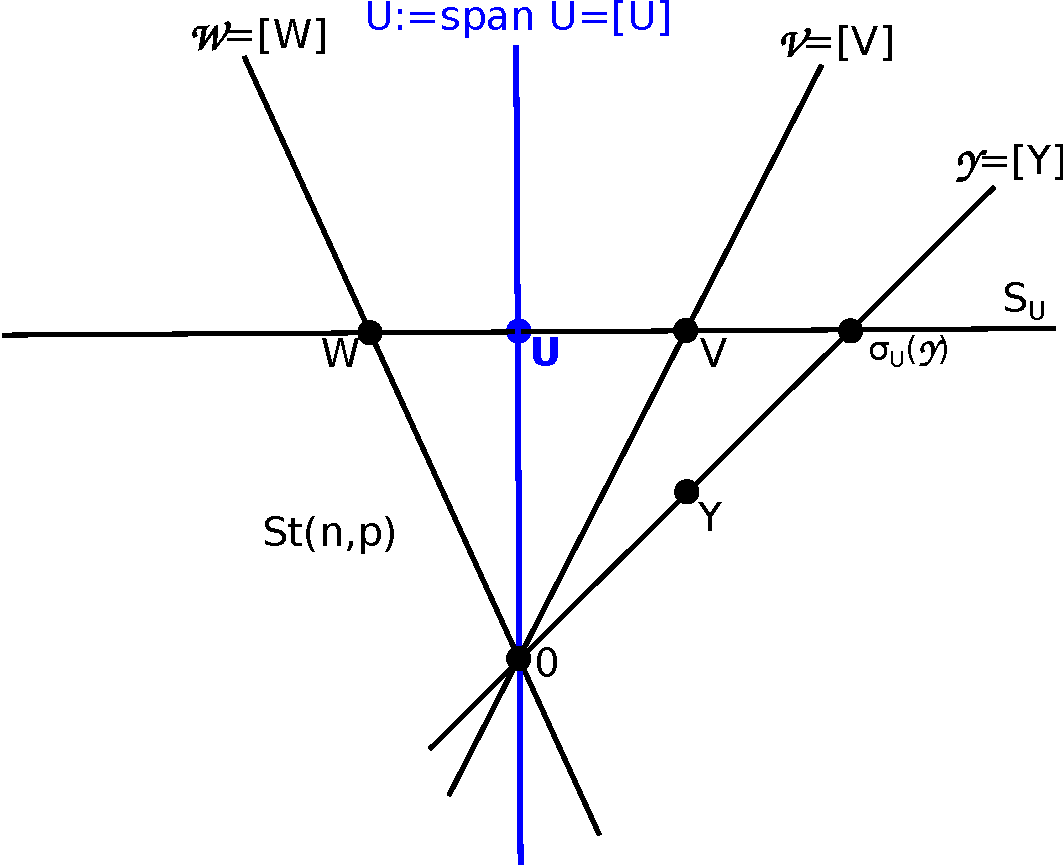
\includegraphics[width=0.5\linewidth]{./figures/theory/affinecrosssection.pdf}
	\caption[Affine cross section map]{ The cross section mapping is illustrated for the special
	case of $St(2,1)\subset\mathbb{R}^2$. Equivalence classes are all lines passing through the origin.
	Pick a $U\in St(2,1)$, then the cross section is given by all $V\in St(2,1)$ for which $U-V$ is
	orthogonal to $U$. This is true for the points $V$ and $W$, representing $\mathcal{V}$ and $\mathcal{W}$,
	respectively, but not for the representative $Y$ of $\mathcal{Y}$. 
	The cross section mapping can be used to obtain a representative $\sigma_U(\mathcal{Y})$ of $\mathcal{Y}$
	which lies again on the cross section. Hence, the cross section is a tool for obtaining a set 
	of locally unique representatives.	
	}
	\label{fig:crosssection}
\end{figure}
As an example for the application of the cross section map, consider the calculation of averages on the
Grassmann manifold. 
\begin{example}[Average]
For the case of an average, take representatives $Y_1,\ldots,Y_n\in St(n,p)$ for $\mathcal{Y}_1,\ldots,\mathcal{Y}_n\in Gr(n,p)$
and find a $U\in St(n,p)$ such that $S_U$ has non-zero intersection with all the $Y_i$'s equivalence classes, which is equivalent
to $U^TY_i\in Gl(p)$. The average $\mathcal{A}$ can then be written as
\begin{equation}
    \mathcal{A} := \pi\left(\sum_{i=1}^{n}\sigma_U(Y_i)\right)=\pi\left(\sum_{i=1}^{n}Y_i(U^{T}Y_i)^{-1}\right).
\end{equation}
\end{example}
% subsubsection Locally unique Representative (end)

\subsubsection{Tangent space} % (fold)
\label{ssub:Tangent space}
The quotient structure makes it necessary to work with representatives such that the usual method for finding the tangent space by differentiating
curves on the manifold cannot be applied. 
Instead one has to start with the "numerator" of the quotient $St(n,p)$. For the Grassmann manifold only tangent vectors of a special subspace of $T_YSt(n,p)$,
the horizontal space, can modify the span of a subspace and exactly those belong to the tangent space of $Gr(n,p)$. 
The notion of modifying and non-modifying tangent vectors can be best understood with the help of Figure \ref{fig:horizontalspace}.\\

\begin{figure}[h!]
        \centering
	    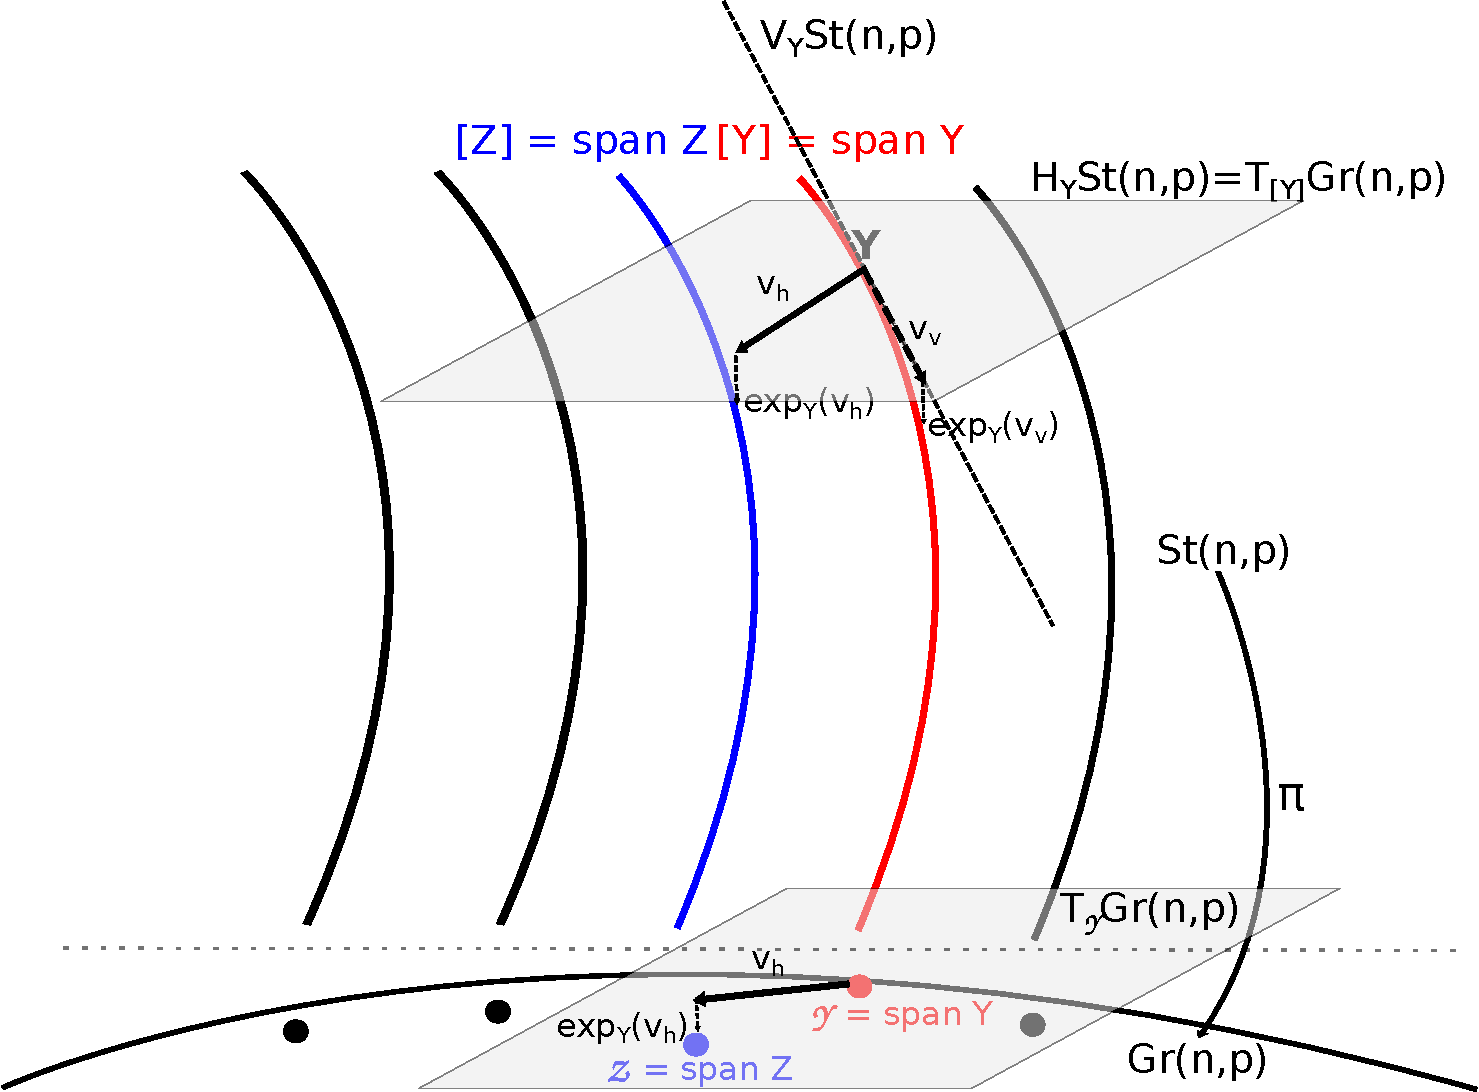
\includegraphics[width=0.6\linewidth]{./figures/theory/quotienttangentspace.pdf}
	\caption[Vertical and horizontal spaces]{ The tangent space $T_YSt(n,p)$ at $Y$ can be decomposed into 
	two parts: The vertical space $V_YSt(n,p)$, defined as the tangent space to the equivalence class (fiber) 
	$[y]=\pi^{-1}(\pi(Y))$, and the horizontal space $H_YSt(n,p)$ as its orthogonal complement. Only tangent vectors of the horizontal space modify the span, 
	in the sense that their retraction (in this case using the exponential map) lies in a different equivalence class.
	Those are the tangent vectors of $T_{\mathcal{Y}}Gr(n,p)$.
	}
	\label{fig:horizontalspace}
\end{figure}


Let $Y\in St(n,p)\subset\mathbb{R}^{n\times p}$. Then the tangent space at $Y$ (\cite{Absil2009} for details of the derivation) to the compact Stiefel manifold is given by
\begin{align}
    \label{eq:stiefel_tangentspace}
   T_YSt(n,p)	&= \left\lbrace Z\in\mathbb{R}^{n\times p}: Y^TZ+Z^TY=0 \right\rbrace\\
   &=  \left\lbrace Y\Omega + Y_{\bot}K: \Omega\in\operatorname{Skew}(p),\, K\in\mathbb{R}^{(n-p)\times p} \right\rbrace\nonumber
\end{align}
where $Y_{\bot}\in\mathbb{R}^{n\times (n-p)}$ is chosen such that $[Y,Y_{\bot}]\in O(n)$. The second representation of (\ref{eq:stiefel_tangentspace})
already implies the decomposition into vertical and horizontal spaces performed in the next steps.\\

The vertical space at $Y$ is by definition the tangent space to the fiber $\pi^{-1}(\pi(Y))$
\begin{equation}
    \label{eq:stiefel_horizontalspace}
    V_Y = T_Y\pi^{-1}(\pi(Y))=T_YY[O(p)]=Y[\operatorname{Skew}(p)],
\end{equation}
while the horizontal space is defined as its orthogonal complement with respect to (\ref{eq:stiefel_tangentspace})
\begin{equation}
    \label{eq:stiefel_verticalspace}
    H_Y=V_Y^{\bot} =\left\lbrace H\in T_Y St(n,p):Y^TH=0 \right\rbrace \simeq Y_{\bot}[\mathbb{R}^{(n-p)\times p}].
\end{equation}

Using this, the tangent space to $Gr(n,p)$ at $\pi(Y)=\mathcal{Y}$, along with its projector, is given by 
\begin{align}
    \label{eq:grassmann_tangentspace}
    T_{\mathcal{Y}}Gr(n,p)&\simeq  H_YSt(n,p)\simeq Y_{\bot}[\mathbb{R}^{(n-p)\times p}]\\
    \pi_{Y_{\bot}}&:=\mathbbm{1}_n-YY^T.
\end{align}

The problem that remains is to pick a unique representative for a tangent vector $\xi\in T_{\mathcal{Y}}Gr(n,p)$.
This is resolved by demanding that the unique representative $\xi_{\Diamond Y}$ should project to $\xi$ via
\begin{equation}
d\pi(Y)\xi_{\Diamond Y}=\xi
\end{equation}
where $\pi: St(n,p)\to Gr(n,p)$ is the canonical quotient projection, such that $d\pi$ is a map between their 
tangent spaces. Using the cross section mapping (\ref{eq:crosssectionmap}), $\xi_{\Diamond Y}$ can be computed by
\begin{equation}
\xi_{\Diamond Y} = d\sigma_Y(\mathcal{Y})\xi.
\end{equation}
$\xi_{\Diamond Y}$ is called the \emph{horizontal lift} of $\xi\in T_{\mathcal{Y}}Gr(n,p)$ at $Y\in St(n,p)$.\\

Finally, to obtain a basis for the tangent space, choose $\left\lbrace E_{ij}\right\rbrace_{i=1,j=1}^{n-p,p}$, with the (i,j)th entry set to one and the rest zero,
as a basis of $\mathbb{R}^{(n-p)\times p}$ and compute $Y_{\bot}$ using a QR decomposition of $Y$. The orthogonal complement $Y_{\bot}$ is then just given by 
$Q_2\in\mathbb{R}^{n\times (n-p)}$ which is part of the decomposition of the orthogonal matrix $Q=[Q_1,Q_2]\in\mathbb{R}^{n\times n}$.\\
For the basis of the tangent space one obtains
\begin{equation}
    \left\lbrace B_{ij}\right\rbrace=\left\lbrace Y_{\bot}E_{ij}\right\rbrace.
\end{equation}

The Riemannian metric for the Grassmann manifold, defined on the tangent space $T_{\mathcal{X}}Gr(n,p)$, is given by 
\begin{equation}
\label{eq:grassmann_metric}
    \braket{R,S}_\mathcal{X} = \tr R^TS,
\end{equation}
which is just the inner product of its embedding space restricted to the manifold.
% subsubection Tangent space (end)

\subsubsection{Exponential map} % (fold)
\label{ssub:Exponential map}
Let $X, R$ span $\mathcal{X}, \mathcal{R}$, respectively and let $U\Sigma V^{T}$ denote the thin singular value decomposition of $R$ with $U\in\mathbb{R}^{n\times p}$, $\Sigma\in\mathbb{R}^{p\times p}$
and $V\in\mathbb{R}^{p\times p}$. Then
\begin{equation}
    \exp_{\mathcal{X}}(\mathcal{R})=\operatorname{span}\left( XV\cos\Sigma V^T + U\sin\Sigma V^T\right).
\end{equation}
% subsubsection Exponential map (end)

\subsubsection{Logarithm map} % (fold)
\label{ssub:Logarithm map}
Let $X, Y$ span $\mathcal{X}, \mathcal{Y}$, respectively and let $U\Sigma V^{T}$ denote the thin singular value decomposition of $Z=\pi_{X_{\bot}}\sigma_X(Y)=(\mathbbm{1}_n-XX^T)Y(X^TY)^{-1}$.
This can be interpreted as choosing a locally unique representative of $Y$ with respect to the affine cross section defined by $X$ and subsequently projecting it back to the tangent space $T_{\mathcal{X}}Gr(n,p)$ at $\mathcal{X}$. 
The map is given by
\begin{equation} 
\log_X(Y) = U\arctan\Sigma V^T. 
\end{equation}

% subsubsection Logarithm map (end)

\subsubsection{Distance function} % (fold)
\label{ssub:Distance function}
Using the exponential map, one can easily define a geodesic distance function on the Grassmann manifold which is induced by its Riemannian metric \ref{eq:grassmann_metric}. The distance function is given by the principal angles $\theta_i$ between the subspaces 
\begin{equation}
    \label{eq:gr_geod_dist}
    d_g^2(X,Y) = \norm{\theta}_2^2=\sum_{i=1}^p\theta_i^2,
\end{equation}
where the the principal angles can be obtained by computing the singular value decomposition of $X^TY$.

\begin{align}
    X^TY &= U\Sigma V^T = U\cos\Theta V^T\\
    \Sigma &= \operatorname{diag} (\sigma_1,\cdots,\sigma_p)\\
    \Theta &= \operatorname{diag} (\theta_1,\cdots,\theta_p) = \operatorname{diag} (\arccos\sigma_1,\cdots,\arccos\sigma_p).
\end{align}

The distance function (\ref{eq:gr_geod_dist}) has the disadvantage that due to the occurrence of the arccosine
and the singular value decomposition, analytic expression are much harder to obtain.\\

To avoid this problem, following Absil's \cite{AbsilGrassmann} approach, an equivalent norm can be chosen, the so-called projection Frobenius norm, given by

\begin{equation}
    d_P^2(X,Y) = \frac{1}{2}\norm{XX^T-YY^T}_{F}^{2} = \sum_{i=1}^p\sin^2\theta_i.
\end{equation}


% subsubsection Distance function (end)


\subsubsection{First derivatives of the distance function} % (fold)
\label{ssub:First derivatives of the distance function}

\begin{equation}
    \label{eq:gr_x_der}
    \frac{\partial d^2(X,Y)}{\partial X} = 2\left(XX^T-YY^T\right)X.
\end{equation}


% subsubsection First derivatives of the distance function (end)

\subsubsection{Second derivatives of the distance function} % (fold)
\label{ssub:Second derivatives of the distance function}

\begin{equation}
    \label{eq:gr_xx_der}
    \frac{\partial^2 d^2(X,Y)}{\partial X\partial X} = 2
    \left[
	\left(X^TX\otimes \mathbbm{1}_{n}\right) 
	+ \left(\mathbbm{1}_p\otimes (XX^T-YY^T)\right)
	+ \left(X^T\otimes X\right)K_{np}
    \right].
\end{equation}

The mixed derivative is given by
\begin{equation}
    \label{eq:gr_xy_der}
    \frac{\partial^2 d^2(X,Y)}{\partial X\partial Y} = -2\left[\left(X^TY\otimes \mathbbm{1}_{n}\right) + \left(X^T\otimes Y\right)K_{np}\right].
\end{equation}


% subsubsection Second derivatives of the distance function (end)


% subsection Grassmanian Gr(N,P) (end)

% section Manifolds (end)

\section{Fr\'{e}chet derivatives of matrix logarithm and square root} % (fold)
\label{sec:frechetderivatives}
To use the derivative expressions computed above, one needs the so-called Kronecker form of the Fr\'{e}chet derivative. The Fr\'{e}chet derivative
of a matrix valued function $f:\mathbb{R}^{n\times n}\to\mathbb{R}^{n\times n}$ at a point $X\in\mathbb{R}^{n\times n}$ is a linear function mapping $E\in\mathbb{R}^{n\times n}$
to $L_f(X,E)\in \mathbb{R}^{n\times n}$ such that
\begin{equation}
    f(X+E) - f(X) - L_f(X,E) = o(\norm{E}).
\end{equation}
Chain rule and inverse function theorem also hold for the Fr\'{e}chet derivative:
\begin{align}
    L_{f\circ g}(X, E) &= L_{f}(g(X)),L_{g}(X,E))\\
    L_{f}(X, L_{f^{-1}}(f(X),E)) &= E.
\end{align}

As the formulation of the derivatives of the distance function, the Fr\'{e}chet derivative can also be brought in the Kronecker form in which it is represented as map
$K_f:\mathbb{R}^{n^2}\to\mathbb{R}^{n^2}$, such that $K_f(X)\in \mathbb{R}^{n^2\times n^2}$ is defined by
\begin{equation}
    \label{eq:kronckerform}
    \operatorname{vec}(L_f(X,E))=K_f(X)\operatorname{vec}(E).
\end{equation}
Here $\operatorname{vec}:\mathbb{R}^{n\times n}\to\mathbb{R}^{n^2}$ denotes the column-wise vectorization operator.

\subsection{Derivative of the matrix square root} % (fold)
\label{sub:Derivative of the matrix square root}
Start by considering the Fr\'{e}chet derivative of $f(X)=X^2$, which is given by
\begin{equation}
    L_{X^2}(X,E) = XE + EX.
\end{equation}
Applying the inverse function theorem consequently leads to
\begin{equation}
    L_{X^2}(X^{\frac{1}{2}},L_{X^{\frac{1}{2}}}(X,E))=X^{\frac{1}{2}}L_{X^{\frac{1}{2}}}(X,E) + L_{X^{\frac{1}{2}}}(X,E)X^{\frac{1}{2}} = E,
\end{equation}
where the last equality shows that the Fr\'{e}chet derivative of the matrix square root $L_{X^{\frac{1}{2}}}(X,E)$ satisfies the Sylvester equation 
\begin{equation}
    \label{eq:sylvester}
    X^{\frac{1}{2}}L + LX^{\frac{1}{2}} = E,\quad L:=L_{X^{\frac{1}{2}}}(X,E).
\end{equation}

The Kronecker representation $K_{X^{\frac{1}{2}}}$ can now be obtained by using the vectorization operator on both sides of the equation and rearrange the term
to the form (\ref{eq:kronckerform}) which leads to
\begin{equation}
	\label{eq:sqrtderivative}
    K_{X^{\frac{1}{2}}}(X)=\left[\left(\mathbbm{1}\otimes X^{\frac{1}{2}}\right)+\left(X^{\frac{1}{2}T}\otimes \mathbbm{1}\right) \right]^{-1}.
\end{equation}

Since the main application of this computation will be for the case $n=3$, (\ref{eq:sqrtderivative}) can
be directly implemented by explicitly calculating the inverse of the $9 \times 9$ matrix $\left(\mathbbm{1}\otimes X^{\frac{1}{2}}\right)+\left(X^{\frac{1}{2}T}\otimes \mathbbm{1}\right)$.\\

For general applications with much larger $n$, however, this approach has the disadvantage that the inverse of a $n^2\times n^2$ matrix needs to be computed, which has computational complexity
$\mathcal{O}((n^2)^3)=\mathcal{O}(n^6)$. In that case, it might be favorable to choose a basis for $\mathbb{R}^{n\times n}$ and solve the Sylvester equation (\ref{eq:sylvester}) for each of the $n^2$ basis matrix elements individually. This is shown for the Kronecker representation of the matrix logarithm in the next section.

%This complexity might eventually be improved considering the 
%special structure of the matrix with 
%
%
%In addition to that, the inverse needs to be found explicitly which is not numerically stable in general.\\
%
%The Sylvester equation (\ref{eq:sylvester}), on the other hand, can be solved with $\mathcal{O}(n^3)$ operations via Schur transformation. Choose $E^{ij}$, the single-entry
%matrices having 1 at $(i,j)$ and zero everywhere else, as a basis for $\mathbb{R}^{n\times n}$ and solve the Sylvester equation for each of the $n^2$ 
%basis matrix elements. By that, the total complexity can be reduced to $n^2\mathcal{O}(n^3)=\mathcal{O}(n^5)$ and the 
%potentially problematic explicit computation of inverses avoided altogether.\\
%
%Some restrictions apply to this simple complexity analysis. Firstly, $\left(\mathbbm{1}\otimes X^{\frac{1}{2}}\right)+\left(X^{\frac{1}{2}T}\otimes \mathbbm{1}\right)$ has a special structure such that it has a maximum of $\mathcal{O}(4)$ distinct entries
%and might be also sparse depending on the structure of $X^{\frac{1}{2}}$. Using a solver exploiting this special structure,
%the complexity of $\mathcal{O}(n^6)$ can eventually be improved. Secondly, since the main application of the algorithm
%will be for the case $n=3$, asymptotic behavior is not that indicative for the real performance of these alternatives,
%which should consequently be measured in more detail for all the relevant small-$n$ cases. \\



\subsection{Derivative of the matrix logarithm} % (fold)
\label{sub:Derivative of the matrix logarithm}
For the logarithm, the implementation follows the approach described by Al-Mohy et al \cite{AlmohyFrechet} 
which is based on the differentiation of the Pad\'{e} approximant to $\log(1+X)$.
Since the application is only valid if the spectral radius of $X$ is sufficiently small, the  use of an inverse scaling and squaring technique based on the relation
\begin{equation}
    \log(X) = 2\log(X^{\frac{1}{2}})
\end{equation}
is necessary.\\

Application of the chain rule leads to
\begin{equation}
    L_{\log}(X,E_0) = 2\log\left(X^{\frac{1}{2}},L_{X^{\frac{1}{2}}}(X,E_0)\right).
\end{equation}
The second argument on the right hand side can again be written as solution $E_1:=L_{X^{\frac{1}{2}}}(A,E_0)$ of an Sylvester-type equation
\begin{equation}
    X^{\frac{1}{2}}E_1+E_{1}X^{\frac{1}{2}}=E_0.
\end{equation}
Repeating the procedure $s$ times results in
\begin{align}
    L_{\log}(X,E_0)&=2^sL_{\log}\left(X^{\frac{1}{2^s}},E_s\right)\\
    X^{\frac{1}{2^{i}}}E_i+E_iX^{\frac{1}{2^{i}}}&=E_{i-1},\quad i=1,\ldots,s
\end{align}
where $E_s$ is obtained by successively solving the set of Sylvester equations defined in the second line.\\

Finally, the Pad\'{e} approximant of order $m$ in its partial fraction form \cite{HighamPade} is given by
\begin{equation}
    \label{eq:pade_log}
    r_m(X) = \sum_{j=1}^{m}\alpha_j^{(m)}(\mathbbm{1}+\beta_j^{(m)}X)^{-1}X
\end{equation}
where $\alpha_{j}^{(m)},\beta_{j}^{(m)}\in (0,1)$ are the $m$-point Gauss-Legendre quadrature weights and nodes.\\

The derivative of (\ref{eq:pade_log}) is then easily computed as 
\begin{equation}
    L_{r_m}(X,E) = \sum_{j=1}^m\alpha_j^{(m)}(\mathbbm{1}+\beta_j^{(m)}X)^{-1}E(\mathbbm{1}+\beta_j^{(m)}X)^{-1}
\end{equation}
which leads to the final approximation of the matrix logarithm derivative, 
\begin{equation}
    \label{eq:dlog_approx}
    L_{\log}(X,E)\approx 2^{s}L_{r_m}\left(X^{\frac{1}{2^s}}-\mathbbm{1},E_s \right).
\end{equation}

For the implementation of (\ref{eq:dlog_approx}), algorithm 5.1 from \cite{AlmohyFrechet} with fixed $m=7$ is used.\\

Choose $E^{ij}$, the single-entry
matrices having 1 at $(i,j)$ and zero everywhere else, as a basis for $\mathbb{R}^{n\times n}$ and compute the
Fr\'{e}chet derivative for every $E^{ij}$. Then, by constructing its rows from the vectorized, transposed Fr\'{e}chet derivatives, the final Kronecker form of the derivative can be obtained by
\begin{equation}
    \left(K_{\log X}\right)_{in + j,\cdot} = \operatorname{vec}\left(L_{\log}(X,E^{ij})^T\right).
\end{equation}
% subsection Derivative of the matrix logarithm (end)




% subsection Derivative of the matrix square root (end)


% section Frechet derivative of the matrix logarithm and square root (end)


\end{chapter}
